
\section{Background}

\subsection{Artificial Neural Networks}
Neural networks are a type of computational model that is inspired by the way brains function. Artificial neural networks are made up of component nodes which are stacked into layers and connected to form a network (see Figure \ref{fig:neural-network}). The neural network operation consists of providing input data to the input layer of the network, passing that data along to network to the output layer and then interpreting the output in a specific way. In the case of predator vs prey, output neurons will correspond to different actions that the predator and prey can make.

\begin{figure}
  \centering
  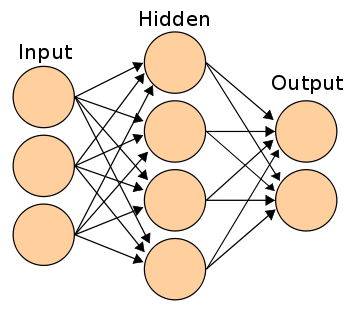
\includegraphics[width=0.5\textwidth]{ANN_structure.png}
  \caption{Representation of a neural network}
  \label{fig:neural-network}
\end{figure}

\subsubsection{Neurons}
The key component nodes of a neural network are called neurons. The sole job of the neuron is to compute the weighted sum of all of the inputs to the neuron which could be from the input data or from other neurons. The computed value is then passed through an activation function. The layout of a neuron can be visualized in Figure \ref{fig:neuron}.


\begin{figure}
  \centering
  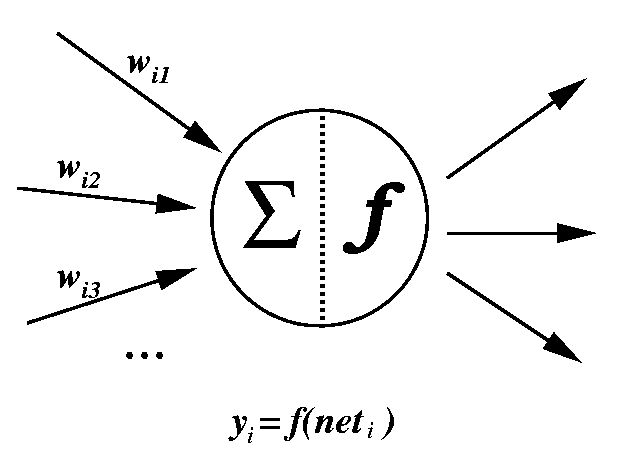
\includegraphics[width=0.5\textwidth]{neuron.png}
  \caption{Representation of a single neuron in a neural network}
  \label{fig:neuron}
\end{figure}

\subsubsection{Activation Functions}
In neural network literature there are several common activation functions that used. The three most used ones are the logistic function, tanh function and the rectifier function. These functions can be seen in Figure \ref{fig:activation-functions} along with their respective formulas. For the purposes of this thesis all activation functions used are the logistic function.



\begin{figure}
  \centering
  \begin{subfigure}{0.3\textwidth}
     \centering
     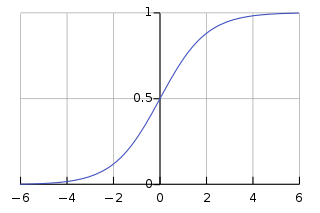
\includegraphics[width=\linewidth]{sigmoid.png}
     \captionsetup{singlelinecheck=off}
     \caption[.]{
     
        \begin{displaymath}
        y = \frac{1}{1+e^(-x)}
        \end{displaymath}}
        logistic function
    }
  \end{subfigure}
  \begin{subfigure}{0.3\textwidth}
     \centering
     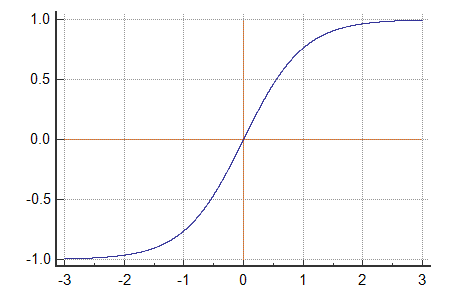
\includegraphics[width=\linewidth]{tanh.png}
     \captionsetup{singlelinecheck=off}
     \caption[.]{
     
        \begin{displaymath}
        y =tanh(x)
        \end{displaymath}}
        tanh function
    }
  \end{subfigure}
  \begin{subfigure}{0.3\textwidth}
   
     \centering
     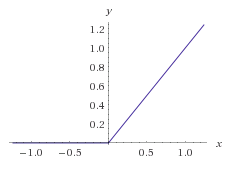
\includegraphics[width=\linewidth]{relu.png}
     \captionsetup{singlelinecheck=off}
     \caption[.]{
        \begin{displaymath}
        y = f(x)=max(0,x)
        \end{displaymath}}
        rectifier function
    }
  \end{subfigure}
  \caption{Common Activation Functions   \label{fig:activation-functions}}
  \end{figure}





\subsection{Particle Swarm Optimization}
\subsubsection{Base PSO Overview}
Particle swarm optimization(PSO) was developed by Kennedy and Eberhart (1995). PSO takes inspiration from the flocking behaviour of swarms of birds. When observing birds there tends to be one leader and the rest of the flock tend to follow that leader. Particles which are analogous to birds are spread throughout a continuous solution space where the particle with the best solution to the problem becomes the leader (global best). Throughout multiple generational time steps the rest of the particles converge towards the global best. If a new best solution is found, the particle that found the new best solution becomes the global best and the process continues until convergence or a max generation cap is reached. This technique allows for a spread out simultaneous search over the search space. 

\subsubsection{Particle}
The particle is the base unit of the PSO. It contains a position within the search space and a velocity. In addition, particles also keep track of their best position until the current time step. This location is the location that has provided the most optimal solution thus far. In the beginning of the algorithm, both the position and the velocity are randomized. This allows the particles to be spread throughout the search space. As the PSO algorithm runs, the particles will move towards the best location, searching the search space along the way.

Each particle also contains a social and cognitive coefficient along with an inertial coefficient that influence how the particle behaves. The social coefficient modifies the influence of the global best position, while the cognitive coefficient modifies the influence of the personal best location. The inertial coefficient modifies the amount of the previous velocity that is carried over to the next time step. These coefficients are used in the velocity update formula, and tend to be picked according to the graph in Figure \ref{fig:pso-convergence} that was proven to be convergent by \cite{englebrecht-pso}.

\begin{figure}
  \centering
  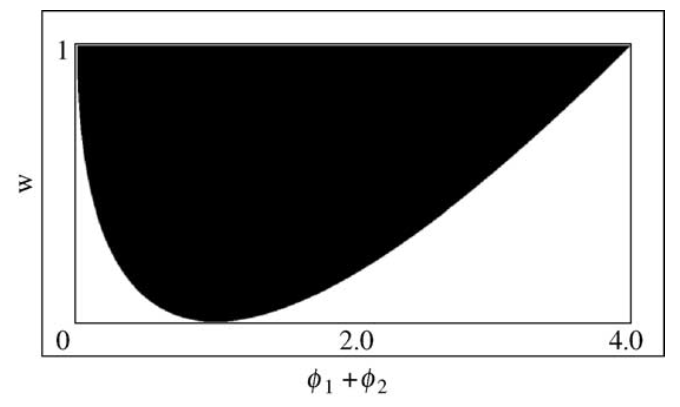
\includegraphics[width=0.5\textwidth]{pso-conv.png}
  \caption{Parameter convergence graph for PSO}
  \label{fig:pso-convergence}
\end{figure}

\subsubsection{Particle Position Update}
The particle position update can be considered as a simplified representation of the concept of motion is classical mechanics. Since each particle contains a velocity vector that represents the direction and magnitude that the particle will move in, that velocity is added to the current position of the particle causing it to move to a different location. The formula is as follows:
\begin{equation} \label{eqn:loc-update}
 x(t+1) = x(t) + v(t)
\end{equation}
where:\\
\indent $x$ represents the position of the particle\\
\indent $v$ represents the velocity of the particle

\subsubsection{Particle Velocity Update}
Each time step, the velocity of the particle is also updated to take into account the particle's current location. In each time step as particles move, the particle's personal best location and the swarm's global best solution could have changed. Therefore, the velocity update formula must take this into account. Another concept that is utilized in the velocity update formula is the idea of inertia from physics. If an object is moving in a certain direction, the object would like to keep moving in that direction unless acted on by another force. This means that if a different force is applied, then the velocity will become the sum of the two forces. When visualized, this causes a smother motion to the particles allowing them to cover more of the search space. The velocity update formula follows below:

\begin{equation} \label{eqn:vel-update-formula}
  v(t+1) = \omega v(t) + c_1 \psi_1  (p(t) - x(t)) + c_2 \psi_2  (g(t) - x(t)) 
\end{equation}
where:\\
\indent $v$ is the velocity of the particle\\
\indent $\omega$ is the inertia coefficient\\
\indent $c_1$ and $c_2$ are the personal and social coefficients respectively\\
\indent $\psi$ is a random multiplier between 0 and 1\\
\indent $x(t)$ is the location of the particle at time t\\
\indent $p(t)$ is the personal best location of the particle at time t\\
\indent $g(t)$ is the global best location of the swarm at time t



%\end{equation}

\subsubsection{Particle Evaluation}
Particle evaluation is problem dependent. For general benchmarking and testing, functions such as the Ackley function and Eggholder function are used to calculate the fitness. The evaluation function for the particles that are used for the predator vs prey problem will be described in depth in section \ref{sec:calc-fitness}.

\subsubsection{Swarms}
Swarms are the major force behind the PSO. A swarm consists of a population of particles. Each swarm is responsible for maintaining the global best position among all of its particles. This is the same value that is used in the velocity update formula. The PSO algorithm could make use of multiple swarms when using algorithms such as the Co-operative Particle Swarm Optimization or Competitive Particle Swarm Optimization algorithms.

The pseudocode for the PSO algorithm can be seen in Figure \ref{fig:pso-pseudocode}.

\subsection{Charged PSO}
\subsubsection{Charged PSO Overview}
Charged PSO is a variation on the normal PSO algorithm. This variation introduces charged particles in order to prevent full convergence and to reduce convergence speed in general. The original PSO algorithm works well for static environments, however it falls short in dynamic environments. As the charged PSO does not fully converge, it is more suitable for dynamic environments with constantly changing error landscapes.

\subsubsection{Charged Particles and Updating}
The introduction of charged particles is the defining feature of charged PSO. Similarly to the original PSO particle, charged particles also contain a position, velocity and personal best location, however they also carry a charge. This charge can differ from particle to particle. 

%\subsubsection{Charged Particle Position Update}
The charged particle's position update formula is the addition of the velocity to the particle's current location. This formula is identical to the normal PSO's particle position update equation.

%\subsubsection{Charged Particle Velocity Update}
The charged particle's velocity update formula introduces an additional term to the formula seen in the normal particle velocity update formula. The new velocity update formula is as follows:

\begin{equation} \label{eqn:charged-vel-update}
 v(t+1) = \omega v(t) + c_1\psi_1 (p(t) - x(t)) + c_2 \psi_2  (g(t) - x(t)) + a_i(t)
\end{equation} This introduces the term $a_i(t)$ to Formula \ref{eqn:vel-update-formula} which a force that is calculated for each particle and is the repulsion force that a charged particle feels from other charged particles in the area. The repulsion force is given by the formula:

\begin{equation} \label{eqn:a-def}
 a_i(t) = \sum_{j=1, j\neq i}^{n_s} a_{ij}(t)
\end{equation}where:
 \begin{equation}\label{eq:a-rules}
a_{ij} = 
    \begin{cases}  
    \frac{Q_{i}Q_{j}}{d_{ij}^3} * (x_{i}(t)-x_{j}(t)) & \text{if  $R_{c} \leq d_{ij} \leq R_{p}$}\\ 
    \frac{ Q_{i}Q_{j} }{R_c^2 d_{ij}}*(x_{i}(t)-x_{j}(t)) & \text{if  $R_{c} < d_{ij}$}\\ 
    0 & \text{otherwise}
    \end{cases}
\end{equation}
where:\\
\indent $d_{ij} = ||(x_{i}(t)-x_{j}(t))||$ or the euclidian distance between particles i and j\\
\indent $Q$ is the charge of the particle \\
\indent $R_{c}$ is the core radius \\
\indent $R_{p}$ is the particle perception limit

This equation can be imagined as a particle surrounded by two fields. If a charged particle is outside the outer field (provided by the perception limit) then the particles are far enough apart from each other that no force is experienced between the particles. Within the perception limit but outside the core radius, the force experienced between the particles scales with the distance. The closer the particles are the more of a repulsion force is experienced. Finally, if the particle is within the core radius limit, the maximum repulsive force is experienced by both particles. This repulsive force ensures that the particle swarm never fully converges. This prevention of full convergence ensures that the PSO can constantly improve in fitness even in dynamic environments.

\subsubsection{Charged Swarms}
Similarly to normal swarms, charged swarms are responsible for the maintenance of the global best position of all the particles in the swarm. Charged swarms can be make up a combination of charged and normal(neutral) particles. As the charged particles interact and repel each other, the charged particles explore the changing landscape searching for better solutions, while the neutral particles provide a more concentrated search around the global best. Since the swarm is also aware of each particle, the charged swarm may also be accountable for calculation the repulsion force experienced by each particle.
 
\begin{figure}
  \centering
  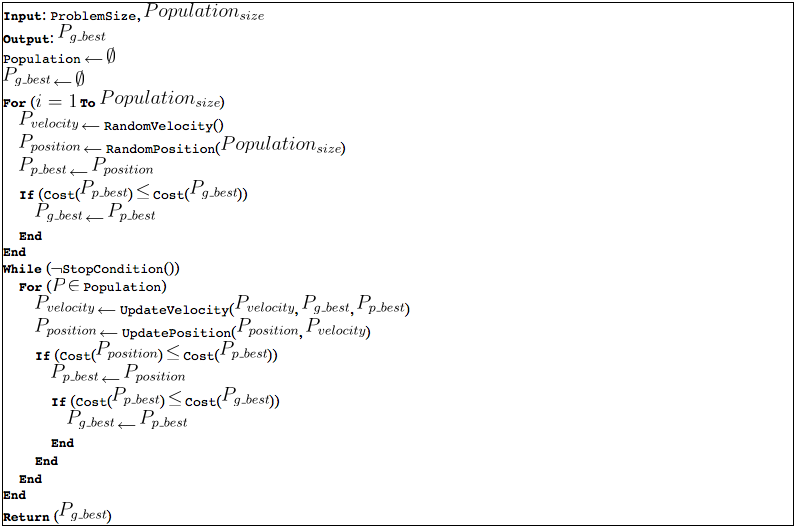
\includegraphics[width=0.8\textwidth]{pso-pseudocode.png}
  \caption{PSO Pseudocode}
  \label{fig:pso-pseudocode}
\end{figure}
	
	


